\documentclass{beamer}
\usetheme{Rochester}
%\usecolortheme{seagull}
%\usecolortheme{whale}
%\setbeamertemplate{footline} % To remove the footer line in all slides uncomment this line
\setbeamertemplate{footline}[page number] % To replace the footer line in all slides with a simple slide count uncomment this line
\setbeamertemplate{navigation symbols}{} % To remove the navigation symbols from the bottom of all slides uncomment this line
\usepackage{graphicx, booktabs,xcolor} 
\usepackage{microtype} % Slightly tweak font spacing for aesthetics
\usepackage{subfiles}
\usepackage{geometry}
\usepackage{multirow}
\usepackage{hyperref}
\usepackage{caption, subcaption}
\usepackage{float}
\usepackage[style=verbose,uniquelist=false,backend=bibtex]{biblatex}
\addbibresource{../myRef.bib}
\renewcommand*{\bibfont}{\scriptsize}
\renewcommand{\footnotesize}{\tiny}

\title{Robot Motion Planning in Dynamic Environment: A Comparative Study}
\author{Dharmin Bakaraniya\footnotemark\\\textbf{Advisors}:\\Prof. Dr. Erwin Prassler\footnotemark\\Dr. Cesar Lopez\footnotemark}
\institute{Hochschule Bonn-Rhein-Sieg}
\date{June 25, 2019}
\begin{document}

\begin{frame}
    \titlepage{}
    \footnotetext[1]{\texttt{dharmin.bakaraniya@smail.inf.h-brs.de}}
    \footnotetext[2]{\texttt{erwin.prassler@h-brs.de}}
    \footnotetext[3]{\texttt{c.a.lopez.martinez@tue.nl}}
\end{frame}

% \begin{frame}
%     \frametitle{\huge{Overview}}
%     \tableofcontents
% \end{frame}

% ==============================================================================
% ==============================================================================
% ==============================================================================
\section{Introduction}
\begin{frame}
    \frametitle{\huge{Introduction I}}
    \begin{columns}[t]
        \column{.50\textwidth}
        \begin{block}{What is motion planning?}
            \begin{itemize}
                \item A mobile robot needs to 
                    \begin{itemize}
                        \item Reach goal in \textbf{minimal} time
                        \item Avoid \textbf{static} \textit{and} \textbf{moving} obstacle
                        \item Consider \textbf{kinematics} \textit{and} \textbf{dynamic} 
                            constraints
                    \end{itemize}
            \end{itemize}
        \end{block}
        \begin{block}{What is our aim?}
            Find out the ``best'' planner
        \end{block}
        \column{.5\textwidth}
        \begin{figure}[htpb]
            \centering
            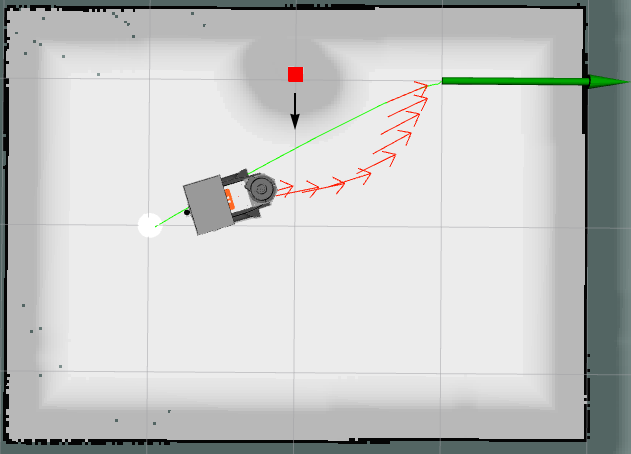
\includegraphics[width=1.0\textwidth]{intro.png}
            \caption{Robot motion planning in dynamic environment}
            \label{fig:intro}
        \end{figure}
    \end{columns}
\end{frame}

% ==============================================================================
\begin{frame}
    \frametitle{\huge{Introduction II}}
    \begin{block}{What are the benefits?}
        \begin{itemize}
            \item \textbf{Safer} environment for humans \textit{and} for robots
            \item \textbf{Cost effective} transportation of goods
        \end{itemize} 
    \end{block}
\end{frame}

% ==============================================================================
% ==============================================================================
% ==============================================================================
\section{State of the art}
\begin{frame}
    \frametitle{\huge{State of the art I}}
    \begin{block}{Survey of motion planning in dynamic environment (2018)~\footcite{mohanan2018a}}
        \begin{itemize}
            \color{blue} \item Covers 101 research papers published between 1985 and 2016
            \color{red}  \item Only introduces approaches. 
            \color{red}  \item Contains almost no comparison.
        \end{itemize}
    \end{block}
\end{frame}

% ==============================================================================
\begin{frame}
    \frametitle{\huge{State of the art II}}
    \begin{block}{Collision avoidance algorithm survey (2015)~\footcite{hoy2015algorithms}}
        \begin{itemize}
            \color{blue} \item Compares collision avoiding algorithms in detail.
            \color{red}  \item Does not validate the comparison with experiments.
            \color{red}  \item Mainly focuses on boundary following algorithms.
        \end{itemize}
    \end{block}
\end{frame}

% ==============================================================================
\begin{frame}
    \frametitle{\huge{State of the art III}}
    \begin{block}{Field contribution survey (2009)~\footcite{keshmiri2009overview}}
        \begin{itemize}
            \color{blue} \item Introduces 150 papers from 1986 to 2008. Compares 
            contribution in different area of motion planning
            \color{red}   \item Only provides contributions of different fields. 
            Does not compare the approaches at all.
        \end{itemize}
    \end{block}
\end{frame}

% ==============================================================================
\begin{frame}
    \frametitle{\huge{State of the art IV}}
    \begin{block}{Dated comparison (1992)~\footcite{hwang1992gross}}
        \begin{itemize}
            \color{blue} \item Surveys papers from 1979 to 1989 for all types of 
            motion planning.
            \color{blue} \item Compares time and complexity
            \color{red} \item Significantly old 
            \color{red} \item Does not compare with common parameters.
        \end{itemize}
    \end{block}
\end{frame}

% ==============================================================================
% ==============================================================================
% ==============================================================================
\section{What is lacking?}
\begin{frame}
    \frametitle{\huge{What is lacking?}}
    \begin{alertblock}{Surveys}
        The surveys do not test the approaches.
    \end{alertblock}
    \begin{alertblock}{Individual published approaches}
        The individual published approaches test themselves
        \begin{itemize}
            \item on \underline{different} robots\footnotemark
            \item with \underline{different} kinodynamic constraints~\footnotemark[8]
            \item with \underline{different} assumptions
            \item in \underline{different} environments 
            \item to optimize \underline{different} parameters~\footnotemark[8]
        \end{itemize}
    \end{alertblock}
    \footcitetext[1]{Michael Hoy; Alexey S. Matveev and Andrey V. Savkin, ``Algorithms for collision-free navigation of mobile robots in complex cluttered environments: a survey'', In: Robotica 33.3 (2015), pp. 463 –497. doi: 10.1017/S0263574714000289.}
\end{frame}

% ==============================================================================
% ==============================================================================
% ==============================================================================
\section{Comparison}
\begin{frame}
    \frametitle{\huge{Qualitative Comparison}}
        We qualitatively compare 30+ planners based on
        \begin{block}{Vehicle type}
            Holonomic, unicycle or bicycle
        \end{block}
        \begin{block}{Restrictions on obstacle}
            \begin{itemize}
                \item Constant or varying direction
                \item Constant or varying velocity
            \end{itemize}
        \end{block}
        \begin{block}{Obstacle shape}
            Circular or polygonal
        \end{block}
        \begin{block}{Experiment environment}
            Simulated and/or real
        \end{block}
\end{frame}


% ==============================================================================
% ==============================================================================
% ==============================================================================
\section{Experimental setup}
\begin{frame}
    \frametitle{\huge{Experimental setup}}
    \begin{block}{Setup}
        \begin{itemize}
            \item \textbf{Robot}: KUKA youBot with 2 laser rangefinders
            \item \textbf{Environment}: Gazebo simulator
            \item \textbf{Obstacle}: Cylinders with varying velocity and varying direction
            \item \textbf{Optimisation parameter}: Minimise time
        \end{itemize}    
    \end{block}
    \begin{columns}
        \column{.45\textwidth}
            \begin{block}{Measured values}
                \begin{itemize}
                    \item Travel time
                    \item Number of collisions
                    \item Number of re-plans
                \end{itemize}
            \end{block}
        \column{.45\textwidth}
        \begin{figure}[htpb]
            \centering
            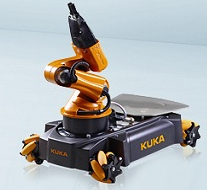
\includegraphics[width=0.7\textwidth]{kuka_youBot.jpg}
        \end{figure}
    \end{columns}
\end{frame}

% ==============================================================================
\begin{frame}
    \frametitle{\huge{Test case 1} (Single room single obstacle)}
    \begin{figure}[ht]
        \centering
        \begin{subfigure}[b]{0.50\linewidth}
            \centering
            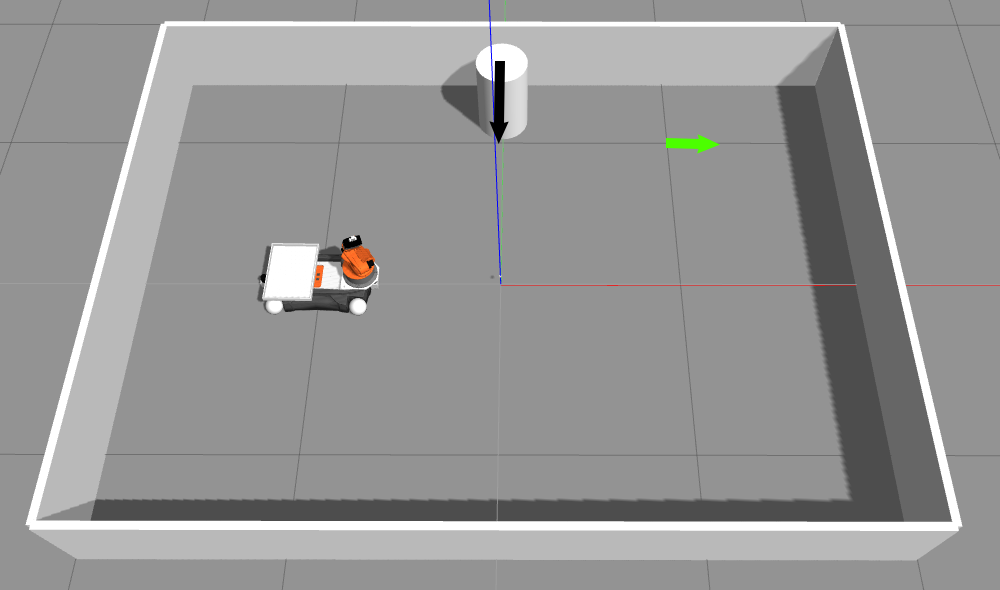
\includegraphics[width=0.95\textwidth]{../report/images/test_case_1/exp1.png}
            \caption{t=0.0s}
        \end{subfigure}%
        \begin{subfigure}[b]{0.50\linewidth}
            \centering
            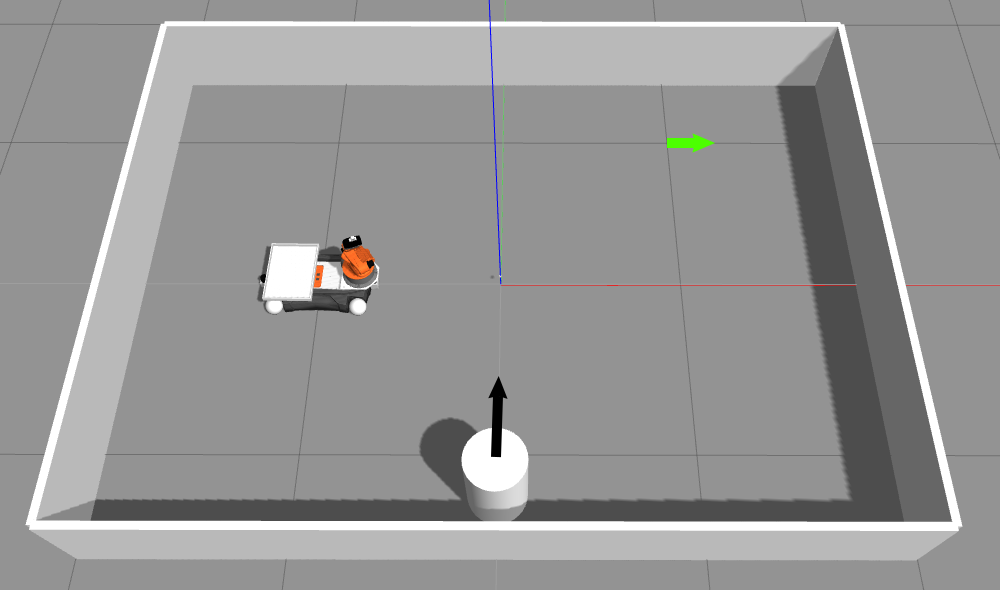
\includegraphics[width=0.95\textwidth]{../report/images/test_case_1/exp3.png}
            \caption{t=10.0s}
        \end{subfigure}%
    \end{figure}
    \begin{block}{Description}
        \begin{itemize}
            \item Room size: 4 meters x 3 meters
            \item Starting position: \texttt{x=-1.0, y=0.0, theta=0.0} 
            \item Goal position: \texttt{x=1.0, y=1.0, theta=0.0}
        \end{itemize}
    \end{block}
\end{frame}

% ==============================================================================
\begin{frame}
    \frametitle{\huge{Test case 2} (Single room two obstacles)}
    \begin{figure}[H]
        \centering
        \begin{subfigure}[b]{0.50\linewidth}
            \centering
            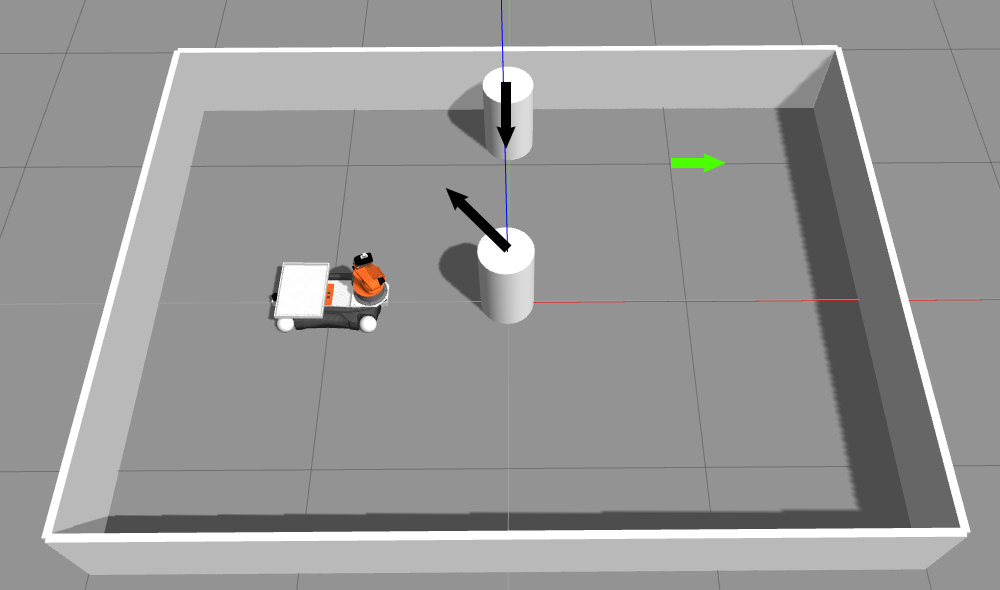
\includegraphics[width=0.90\textwidth]{../report/images/test_case_2/exp1.png}
            \caption{t=0.0s}
        \end{subfigure}%
        \begin{subfigure}[b]{0.50\linewidth}
            \centering
            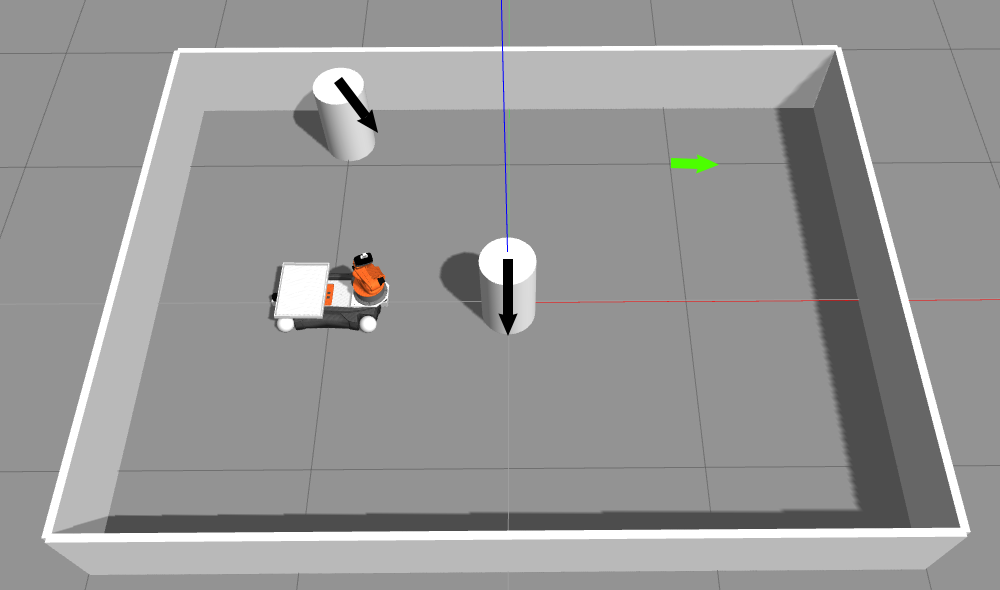
\includegraphics[width=0.90\textwidth]{../report/images/test_case_2/exp2.png}
            \caption{t=5.0s}
        \end{subfigure}
        \begin{subfigure}[b]{0.50\linewidth}
            \centering
            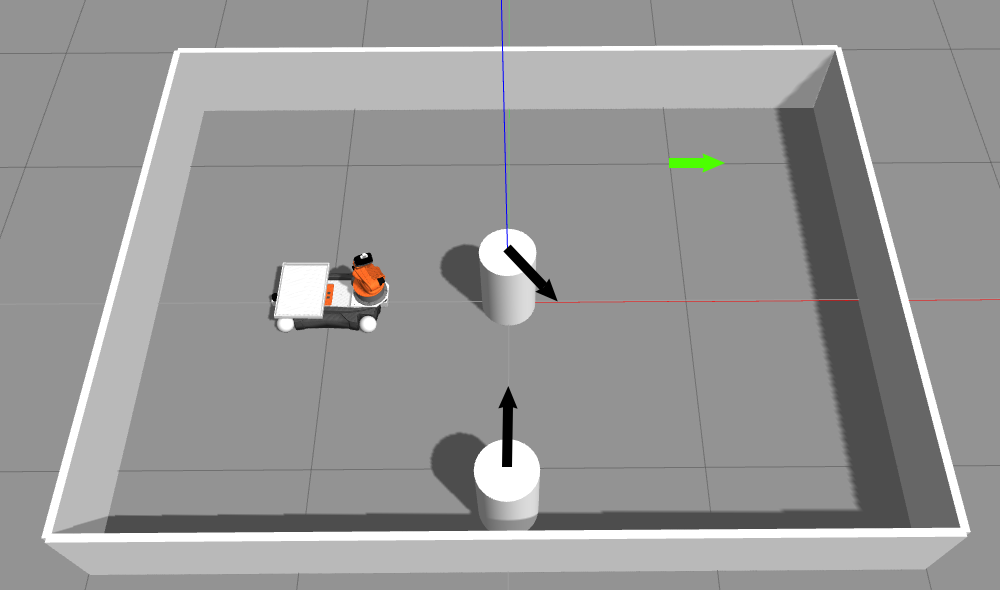
\includegraphics[width=0.90\textwidth]{../report/images/test_case_2/exp3.png}
            \caption{t=10.0s}
        \end{subfigure}%
        \begin{subfigure}[b]{0.50\linewidth}
            \centering
            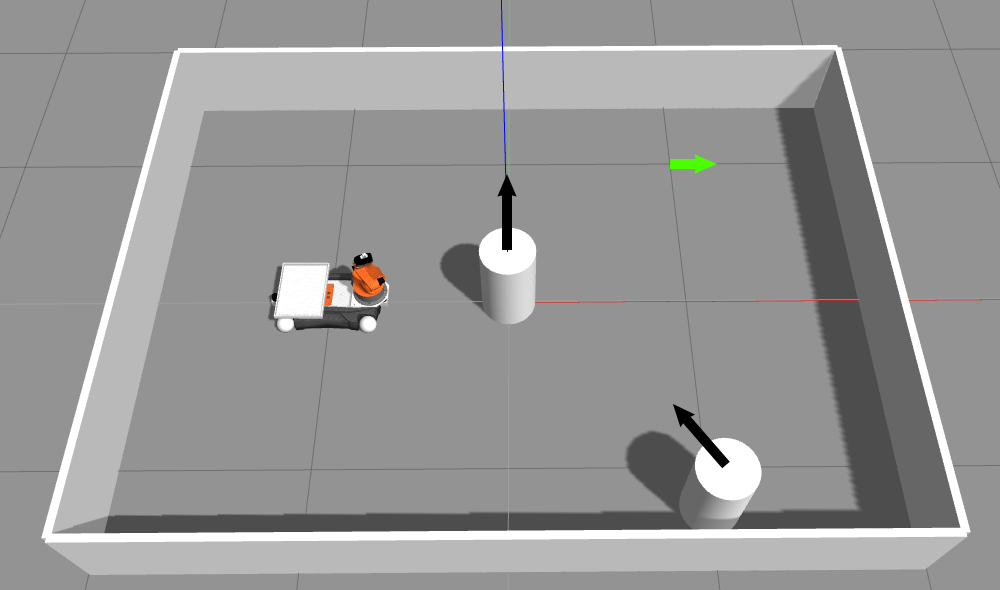
\includegraphics[width=0.90\textwidth]{../report/images/test_case_2/exp4.png}
            \caption{t=15.0s}
        \end{subfigure}%
    \end{figure}
\end{frame}

% ==============================================================================
\begin{frame}
    \frametitle{\huge{Test case 3} (Double room nine obstacles)}
    \begin{figure}[H]
        \centering
        \begin{subfigure}[b]{0.35\linewidth}
            \centering
            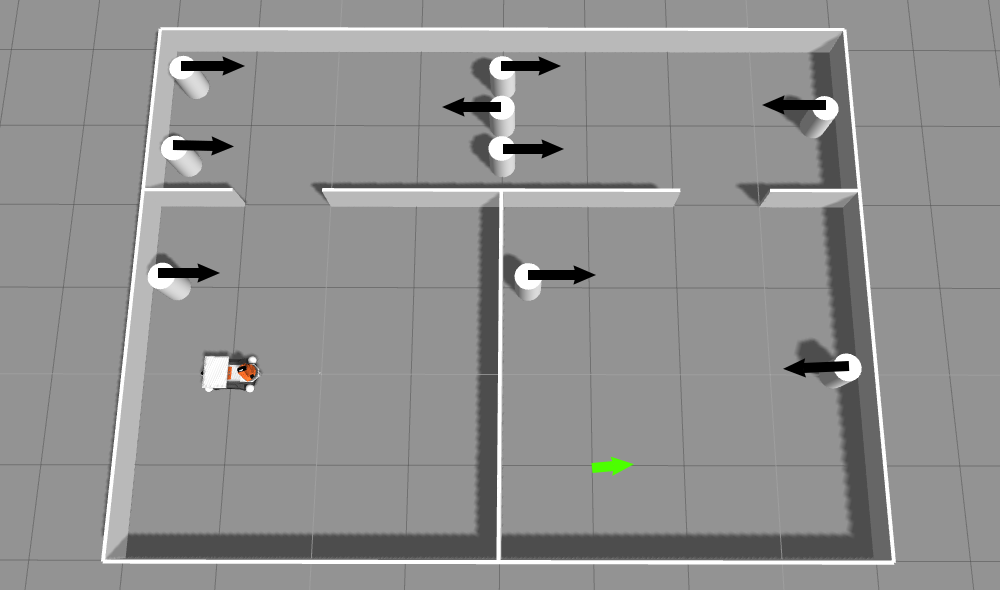
\includegraphics[width=0.95\textwidth]{../report/images/test_case_3/exp1.png}
            \caption{t=0.0s}
        \end{subfigure}%
        \begin{subfigure}[b]{0.35\linewidth}
            \centering
            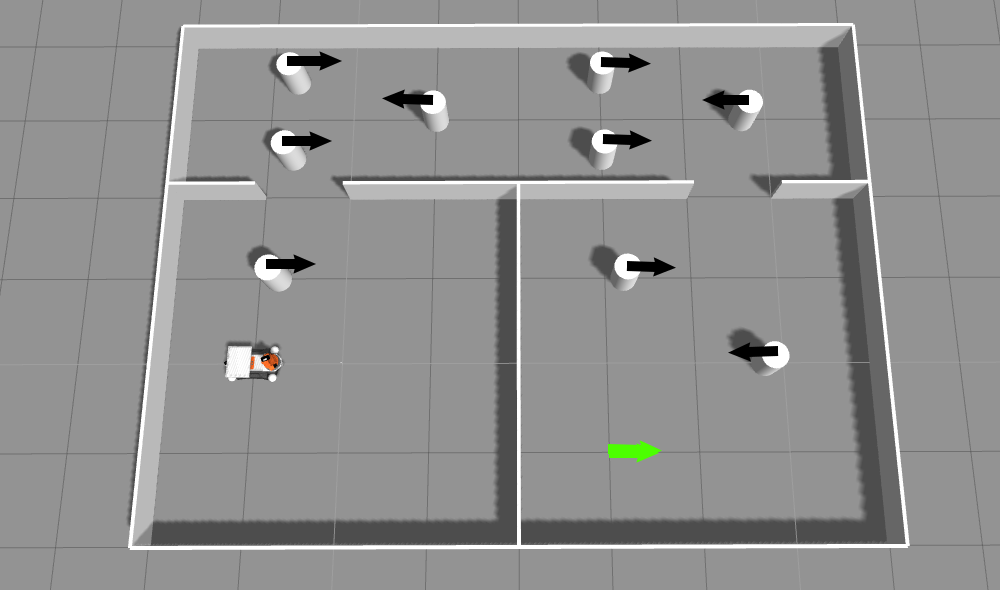
\includegraphics[width=0.95\textwidth]{../report/images/test_case_3/mid1.png}
            \caption{t=5.0s}
        \end{subfigure}%
        \begin{subfigure}[b]{0.35\linewidth}
            \centering
            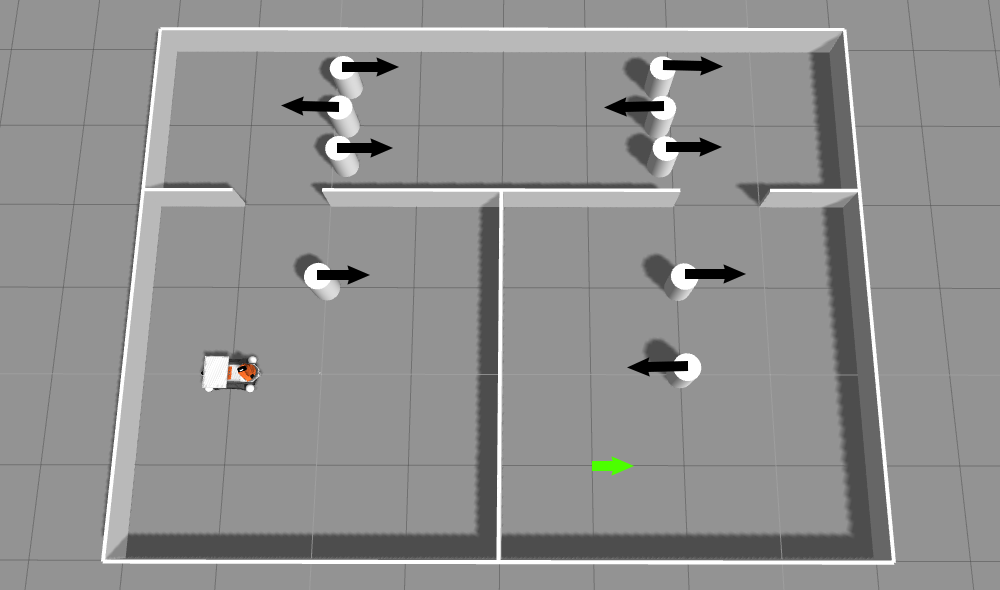
\includegraphics[width=0.95\textwidth]{../report/images/test_case_3/exp2.png}
            \caption{t=7.5s}
        \end{subfigure}
        \begin{subfigure}[b]{0.35\linewidth}
            \centering
            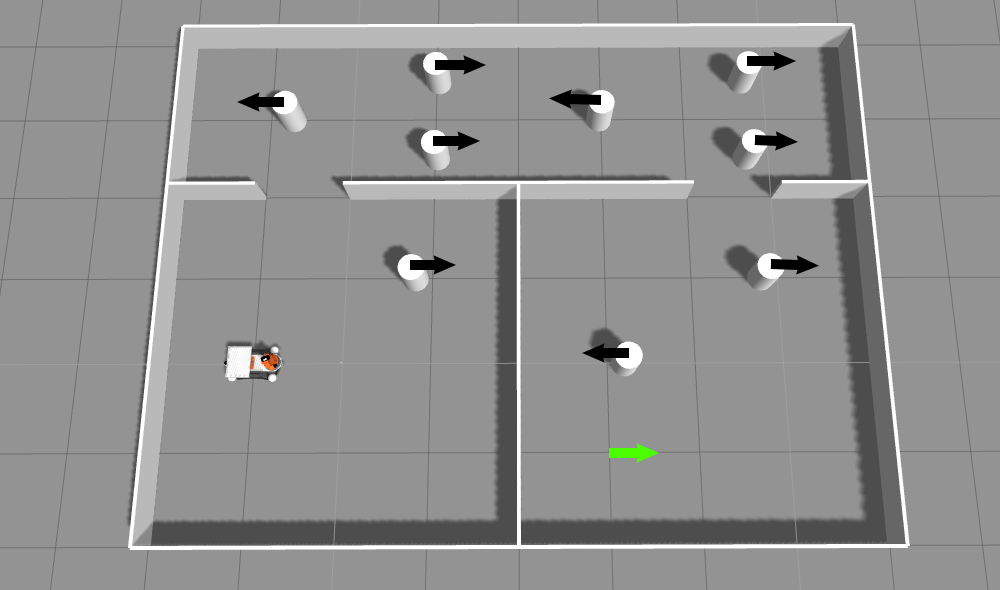
\includegraphics[width=0.95\textwidth]{../report/images/test_case_3/mid2.png}
            \caption{t=10.0s}
        \end{subfigure}%
        \begin{subfigure}[b]{0.35\linewidth}
            \centering
            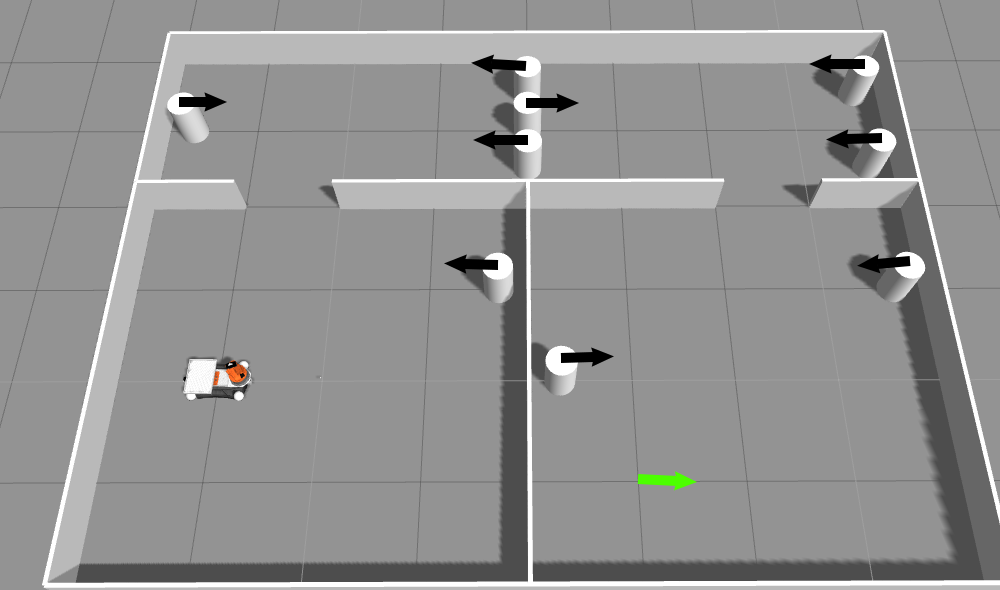
\includegraphics[width=0.95\textwidth]{../report/images/test_case_3/exp3.png}
            \caption{t=15.0s}
        \end{subfigure}%
        \begin{subfigure}[b]{0.35\linewidth}
            \centering
            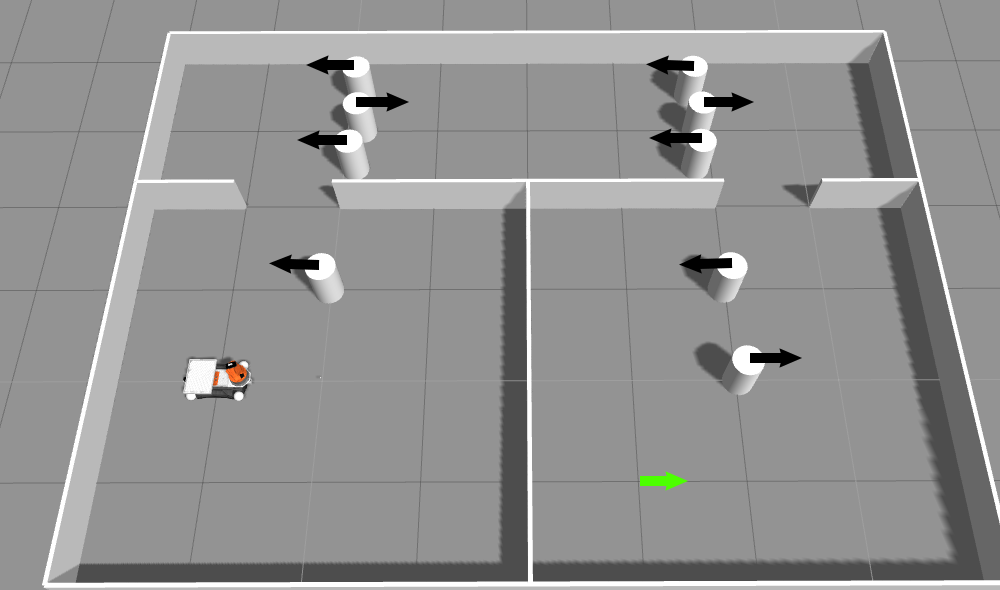
\includegraphics[width=0.95\textwidth]{../report/images/test_case_3/exp4.png}
            \caption{t=22.5s}
        \end{subfigure}
        \caption{Test case 3 (Total size: 8m x 6m)}\label{fig:double_room}
    \end{figure}
\end{frame}

% ==============================================================================
\begin{frame}
    \frametitle{\huge{Compared Planners}}
    \begin{itemize}
        \item Timed elastic band planner (TEB)~\footcite{rosmann2015planning}
        \item Spline based planner\footcite{mercy2017spline}.
        \item Elastic band approach (EBand)\footcite{quinlan1993elastic}.
        \item Eband* (EBand2)
        \item Dynamic window approach* (DWA)~\footcite{fox1997dynamic}
    \end{itemize}
    \tiny{* with obstacle position look ahead of 3 seconds}
\end{frame}

% ==============================================================================
% ==============================================================================
% ==============================================================================
\section{Results}
\begin{frame}
    \frametitle{\huge{Results I (Travel time)}}
    \begin{table}[!htpb]
        \centering
        \begin{tabular}{p{1.5cm}p{1.3cm}p{1.3cm}p{1.3cm}p{1.3cm}p{1.3cm}}\toprule
            \textbf{Planner} & \textbf{Static single room} & \textbf{Test case 1} & \textbf{Test case 2} & \textbf{Static double room} & \textbf{Test case 3} \\\toprule
            \textbf{TEB    } & \textcolor{blue}{\textbf{5.205}}  & 5.972  & 6.083  & \textcolor{blue}{\textbf{27.139}} & \textcolor{blue}{\textbf{35.330}} \\\midrule
            \textbf{Spline } & 5.421  & \textcolor{blue}{\textbf{5.574}}  & \textcolor{blue}{\textbf{5.819}}  & \--    & \--    \\\midrule     
            \textbf{DWA    } & 19.526 & 17.625 & 17.114 & 39.004 & \-- \\\midrule
            \textbf{EBand  } & 6.270  & 6.570  & 6.240  & 30.862 & 71.968 \\\midrule
            \textbf{EBand2 } & 6.270  & 6.025  & 6.234  & 30.862 & \-- \\
            \bottomrule
        \end{tabular}
        \caption{Average time of travel for planners for different test cases}
    \end{table}
\end{frame}

% ==============================================================================
\begin{frame}
    \frametitle{\huge{Results II (Re-plans)}}
    \begin{table}[H]
        \centering
        \begin{tabular}{p{1.5cm}p{1.3cm}p{1.3cm}p{1.3cm}p{1.3cm}p{1.3cm}}\toprule
            \textbf{Planner} & \textbf{Static single room} & \textbf{Test case 1} & \textbf{Test case 2} & \textbf{Static double room} & \textbf{Test case 3} \\\toprule
            \textbf{TEB    } & \textcolor{blue}{\textbf{0}} & \textcolor{blue}{\textbf{0}} & 1 & \textcolor{blue}{\textbf{0}} & \textcolor{blue}{\textbf{4}} \\\midrule
            \textbf{Spline } & \textcolor{blue}{\textbf{0}} & \textcolor{blue}{\textbf{0}} & \textcolor{blue}{\textbf{0}} & Fail & Fail \\\midrule
            \textbf{DWA    } & \textcolor{blue}{\textbf{0}} & \textcolor{blue}{\textbf{0}} & 2 & \textcolor{blue}{\textbf{0}} & Fail \\\midrule
            \textbf{EBand  } & \textcolor{blue}{\textbf{0}} & 1 & Fail & \textcolor{blue}{\textbf{0}} & Fail \\\midrule
            \textbf{EBand2 } & \textcolor{blue}{\textbf{0}} & 1 & 1 & \textcolor{blue}{\textbf{0}} & Fail \\
            \bottomrule
        \end{tabular}
        \caption{Maximum re-plan attempts of planners for different test cases}
    \end{table}
\end{frame}

% ==============================================================================
\begin{frame}
    \frametitle{\huge{Results (collisions)}}
    \begin{table}[H]
        \centering
        \begin{tabular}{p{1.5cm}p{1.3cm}p{1.3cm}p{1.3cm}p{1.3cm}p{1.3cm}}\toprule
            \textbf{Planner} & \textbf{Static single room} & \textbf{Test case 1} & \textbf{Test case 2} & \textbf{Static double room} & \textbf{Test case 3} \\\toprule
            \textbf{TEB    } & \textcolor{blue}{\textbf{0}} & \textcolor{blue}{\textbf{0}} & \textcolor{blue}{\textbf{0}} & \textcolor{blue}{\textbf{0}} & \textcolor{blue}{\textbf{0.75}} \\\midrule
            \textbf{Spline } & \textcolor{blue}{\textbf{0}} & \textcolor{blue}{\textbf{0}} & \textcolor{blue}{\textbf{0}} & \-- & \-- \\\midrule
            \textbf{DWA    } & \textcolor{blue}{\textbf{0}} & \textcolor{blue}{\textbf{0}} & \textcolor{blue}{\textbf{0}} & \textcolor{blue}{\textbf{0}} & \-- \\\midrule
            \textbf{EBand  } & \textcolor{blue}{\textbf{0}} & 0.25 & 0.5 & \textcolor{blue}{\textbf{0}} & 4 \\\midrule
            \textbf{EBand2 } & \textcolor{blue}{\textbf{0}} & \textcolor{blue}{\textbf{0}} & \textcolor{blue}{\textbf{0}} & \textcolor{blue}{\textbf{0}} & \-- \\
            \bottomrule
        \end{tabular}
        \caption{Average collisions of planners for different test cases}
    \end{table}
\end{frame}


% ==============================================================================
\begin{frame}[t]{Results visualised}
    \begin{figure}[H]
        \centering
        \begin{subfigure}[b]{0.450\linewidth}
            \centering
            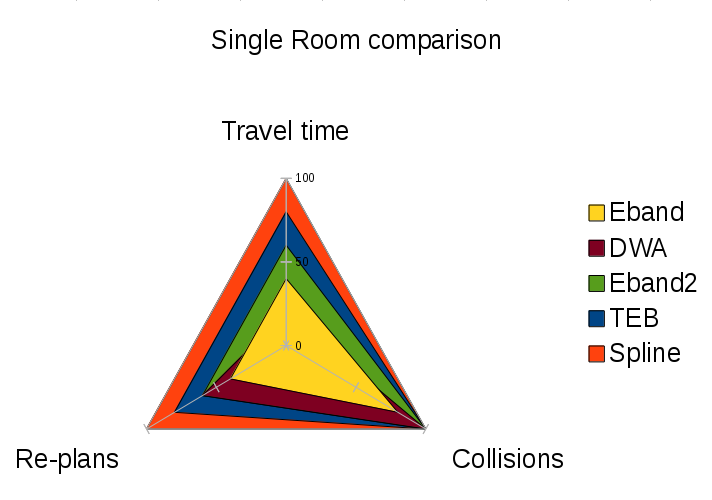
\includegraphics[width=0.99\textwidth]{single_room_web_graph.png}
            \caption{Ranking comparison for test case 1 and 2}
        \end{subfigure}%
        \begin{subfigure}[b]{0.50\linewidth}
            \centering
            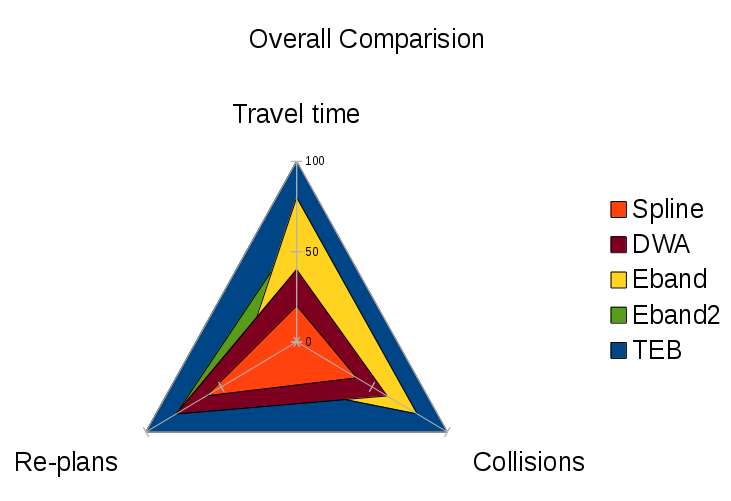
\includegraphics[width=0.99\textwidth]{overall_web_graph.png}
            \caption{Ranking comparison for all test cases}
        \end{subfigure}
    \end{figure}
    \begin{block}{Verdict}
        TEB planner performs best for our experiments out of 5 planners.
    \end{block}
\end{frame}

% ==============================================================================
% ==============================================================================
% ==============================================================================
\section{Conclusion and future work}
\begin{frame}{\huge{Conclusion and future work}}
    \begin{block}{Conclusion}
        \begin{itemize}
            \item Qualitative comparison
            \item Develop an open source software to help test 
            \item Test cases and framework for objective comparison
            \item TEB planner performs ``best'' for given scenarios
        \end{itemize}
    \end{block}
    \begin{block}{Future work}
        \begin{itemize}
            \item Test more planners on these test cases.
            \item Test with humans as obstacles for real robots.
            \item Test with different models of robots.
        \end{itemize}
    \end{block}
\end{frame}

% ==============================================================================
\begin{frame}[allowframebreaks]
    \frametitle{\huge{References}}
    \tiny{ \printbibliography}
\end{frame}
\end{document} 
